\documentclass{article}

\usepackage{graphicx}
\usepackage{tikz}
\usepackage{tikzsymbols}
\usetikzlibrary{calc,patterns,shapes.geometric}
\pagestyle{empty}
\usepackage[margin=0pt]{geometry}
\geometry{papersize={14in,12in}}

\def\centerarc[#1](#2)(#3:#4:#5){\draw[#1] ($(#2)+({#5*cos(#3)},{#5*sin(#3)})$) arc (#3:#4:#5);}

\begin{document}
	\begin{figure}
		\centering
		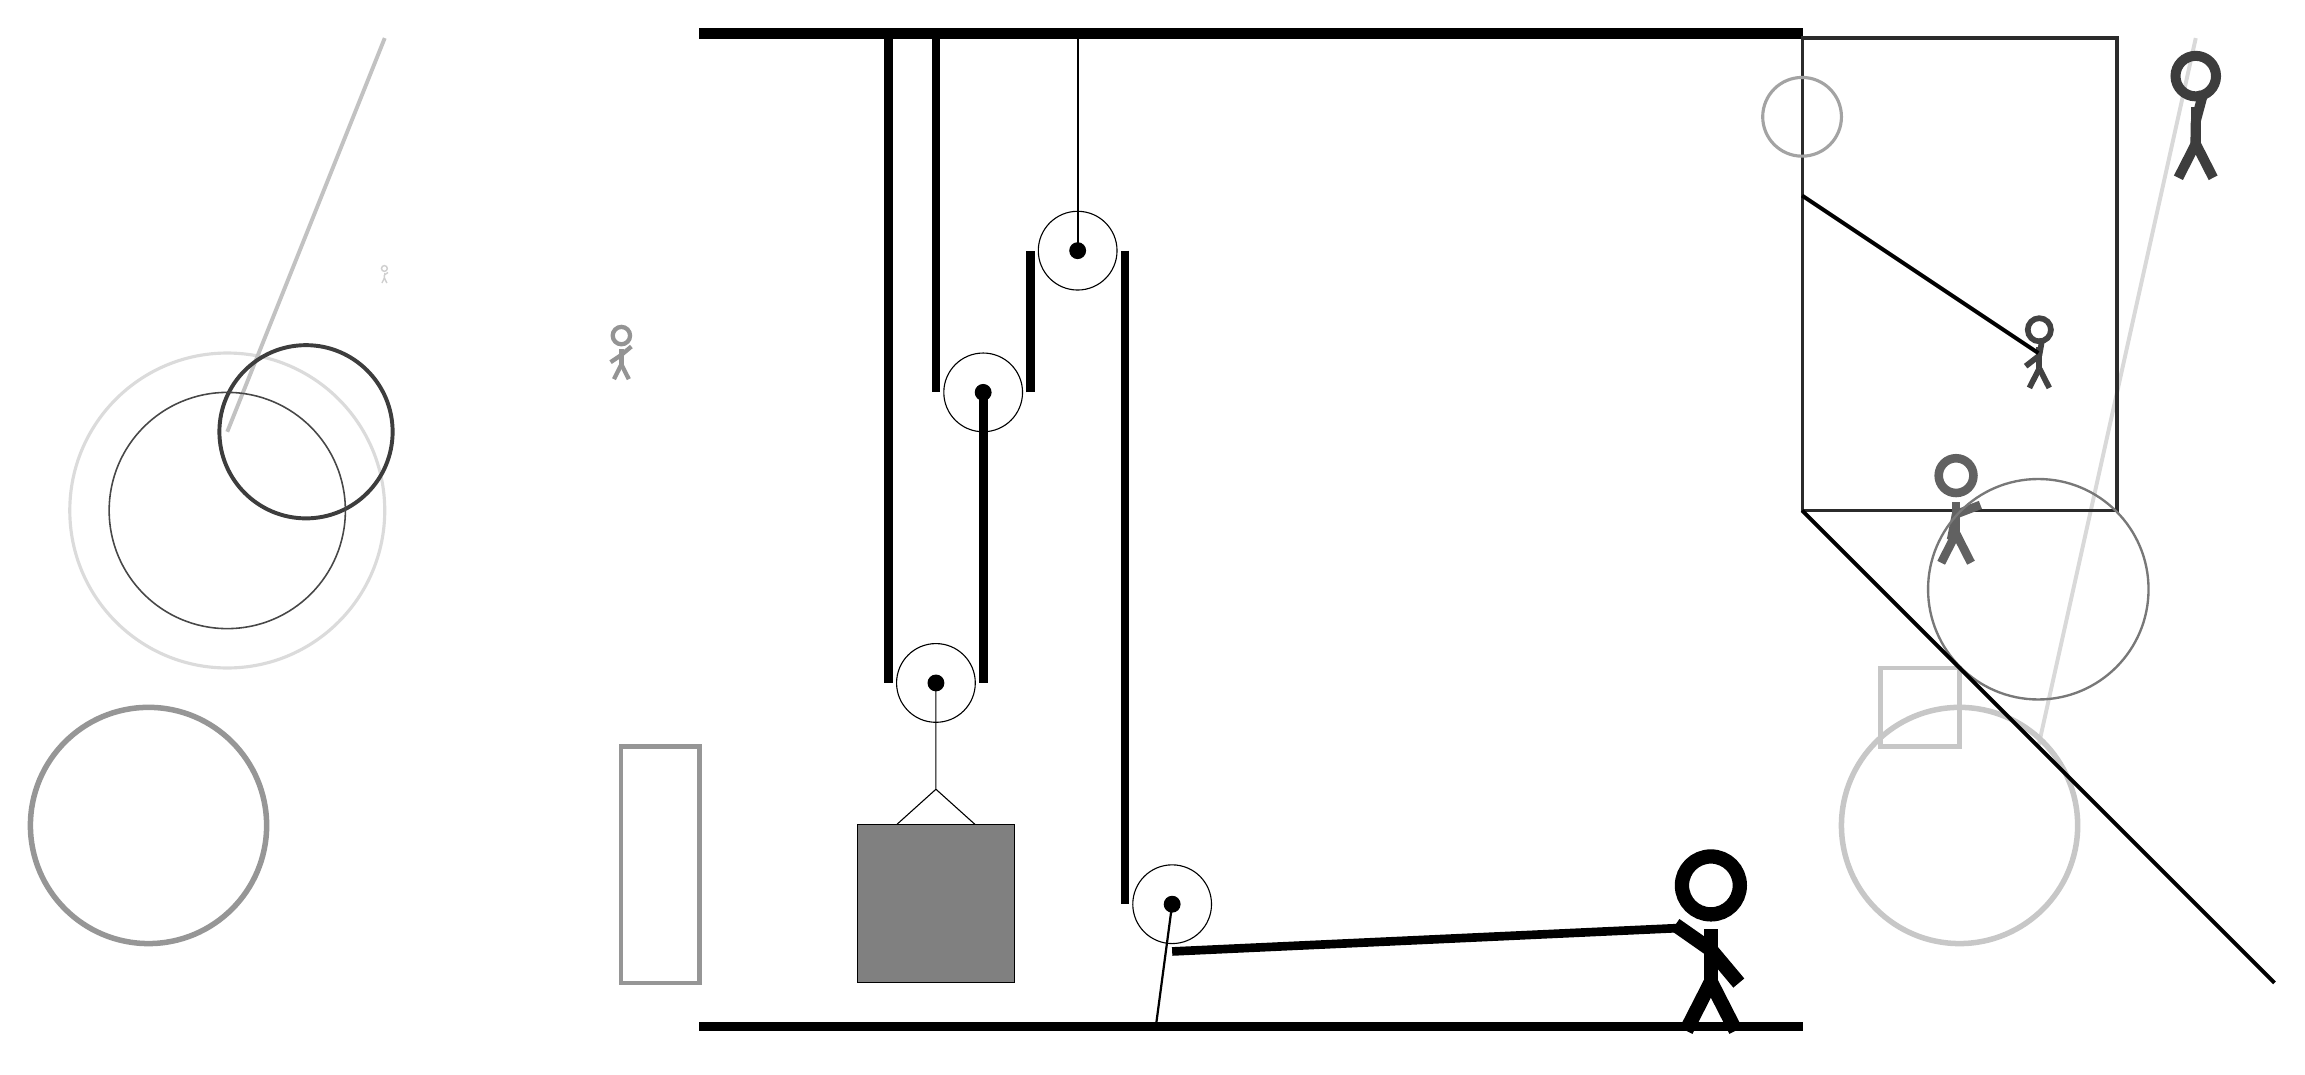
\begin{tikzpicture}
			%%%%% START %%%%%
			
			\draw[fill=black] (-2, 9) rectangle (12, 9.125);
			
			\draw (1, 0.81) circle (0.5);
			\draw[fill=black] (1, 0.81) circle (0.1);
			
			\draw (1.6, 4.5) circle (0.5);
			\draw[fill=black] (1.6, 4.5) circle (0.1);
			
			\draw (2.8, 6.3) circle (0.5);
			\draw[fill=black] (2.8, 6.3) circle (0.1);
			\draw[thick] (2.8, 6.3) -- (2.8, 9);
			
			\draw (4.0, -2) circle (0.5);
			\draw[fill=black] (4.0, -2) circle (0.1);
			\draw[thick] (4.0, -2) -- (3.8, -3.5);
			
			\draw (1, 0.81) -- (1, -0.54) -- (0.5, -0.99) -- (1.5, -0.99) -- (1, -0.54);
			\draw[fill=black!50] (0, -0.99) rectangle (2, -2.99);
			\draw[line width=1.1mm] (0.4, 9) -- (0.4, 0.81);
			\centerarc[line width=1.1mm](1, 0.81)(180:360:0.6);
			\draw[line width=1.1mm](1.6, 0.81) -- (1.6, 4.5);
			\draw[line width=1.1mm] (1.0, 9) -- (1.0, 4.5);
			\centerarc[line width=1.1mm](1.6, 4.5)(180:360:0.6);
			\draw[line width=1.1mm](2.2, 4.5) -- (2.2, 6.3);
			\centerarc[line width=1.1mm](2.8, 6.3)(0:180:0.6);
			\draw[line width=1.1mm] (3.4, 6.3) -- (3.4, -2);
			\centerarc[line width=1.1mm](4.0, -2)(0:90:-0.6);
			\draw[line width=1.1mm](4.0, -2.6) -- (10.5, -2.3);
			
			\draw [line width=0.4mm, color=black!14](-8, 3) circle (2.0);
			
			\draw[line width=0.5mm, color=black!15](17, 9) -- (15, 0);
			\draw[line width=0.4mm, color=black!83] (12, 9) rectangle (16, 3);
			\node[line width=0.7mm, color=black!76] at (17, 8) {\Strichmaxerl[7][89][75]};
			\draw[line width=0.5mm, color=black!24](-6, 9) -- (-8, 4);
			\node[line width=0.3mm, color=black!62] at (14, 3) {\Strichmaxerl[6][79][21]};
			
			\draw [line width=0.7mm, color=black!22](14, -1) circle (1.5);
			
			\draw[line width=0.6mm, color=black!41] (-3, -3) rectangle (-2, 0);
			\draw[line width=0.6mm, color=black!22] (14, 0) rectangle (13, 1);
			\draw [line width=0.5mm, color=black!76](-7, 4) circle (1.1);
			\draw [line width=0.3mm, color=black!53](15, 2) circle (1.4);
			\draw[line width=0.5mm, color=black!100](12, 3) -- (18, -3);
			\draw [line width=0.7mm, color=black!41](-9, -1) circle (1.5);
			\draw [line width=0.2mm, color=black!72](-8, 3) circle (1.5);
			\node[line width=0.5mm, color=black!74] at (15, 5) {\Strichmaxerl[4][38][80]};
			\draw[line width=0.5mm, color=black!100](15, 5) -- (12, 7);
			\draw [line width=0.4mm, color=black!36](12, 8) circle (0.5);
			\node[line width=0.6mm, color=black!42] at (-3, 5) {\Strichmaxerl[3][34][40]};
			\node[line width=0.6mm, color=black!19] at (-6, 6) {\Strichmaxerl[1][89][34]};
			
			
			\node at (10.8, -2.5) {\Strichmaxerl[10][-35][-50]};
			
			\draw[fill=black] (-2, -3.5) rectangle (12, -3.6);
			
			%%%%% END %%%%%
		\end{tikzpicture}
	\end{figure}	
\end{document}